\chapter{Introduction to Qt and SQL Programming\label{ch:Introduction to Qt and SQL Programming}}
So far we have designed the detailed software architecture. Before starting module design and implementation we have to introduce Qt GUI programming and SQL programming.

\section{Qt GUI Programming}
Qt \cite{qt} identifies itself as a cross-platform software development framework. It was originally designed for making graphical user interface applications. The Qt framework consists of the following main modules in Table \ref{tab:Qt Modules} \cite{qtmodules}. As the name indicates, Qt Core is the core of the Qt framework. It defines QObject, the base class of all Qt objects. QObject provides lower-level infrastructure for the Qt Framework and applications.

\begin{table}[htb]
\centering
\caption {Qt Modules\label{tab:Qt Modules}}
\begin{tabular}{p{0.2\textwidth}p{0.75\textwidth}}
\hline
Module & Description \\
\hline
Qt Core & Core non-graphical classes used by other modules. \\ 
Qt GUI & Base classes for graphical user interface (GUI) components. Includes OpenGL. \\
Qt Multimedia & Classes for audio, video, radio and camera functionality. \\
Qt Multimedia \newline Widgets & Widget-based classes for implementing multimedia functionality. \\
Qt Network & Classes to make network programming easier and more portable. \\
Qt QML & Classes for QML and JavaScript languages. \\
Qt Quick & A declarative framework for building highly dynamic applications with custom user interfaces. \\
Qt Quick Controls & Provides lightweight QML types for creating performant user interfaces for desktop, embedded, and mobile devices. These types employ a simple styling architecture and are very efficient. \\
Qt Quick Dialogs & Types for creating and interacting with system dialogs from a Qt Quick application. \\
Qt Quick Layouts & Layouts are items that are used to arrange Qt Quick 2 based items in the user interface. \\
Qt Quick Test & A unit test framework for QML applications, where the test cases are written as JavaScript functions. \\
Qt SQL & Classes for database integration using SQL. \\
Qt Test & Classes for unit testing Qt applications and libraries. \\
Qt Widgets & Classes to extend Qt GUI with C++ widgets. \\
\hline
\end{tabular}
\end{table}

\begin{figure}[htb]
\centering
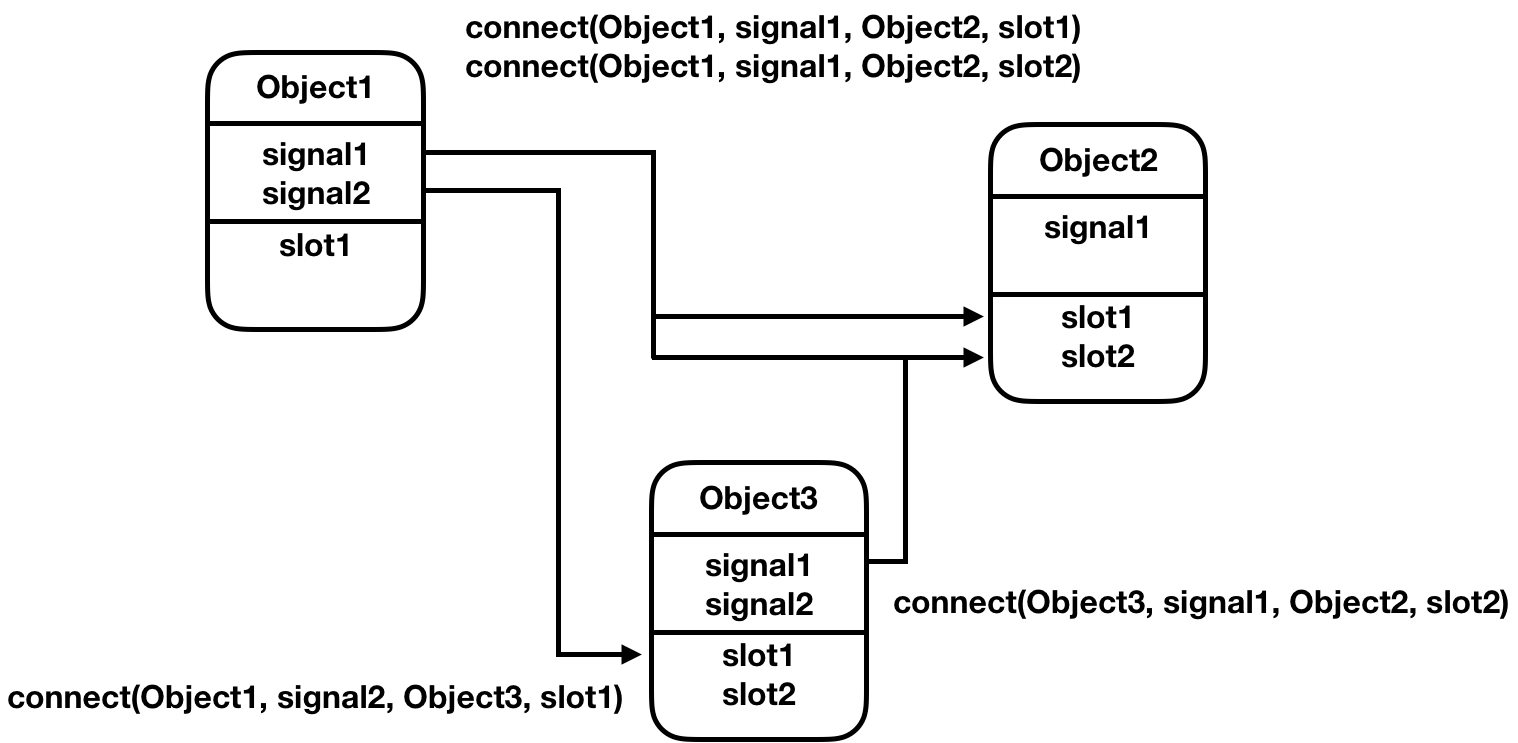
\includegraphics[width = \textwidth]{SignalAndSlot}
\caption{Signal and Slot\label{fig:Signal and Slot}}
\end{figure}

Special attention should be paid to the \textbf{Signal and Slot} \cite{signalsandslots} mechanism supported by QObject. It is a powerful, friendly and intuitive alternative to the callback technique, and is a central feature of Qt. When an event occurs, a signal is emitted. The corresponding slots receive that signal and respond by executing a function. The signal and slot mechanism has three elements: the signal, the slot, and connection between them. They can be illustrated with Figure \ref{fig:Signal and Slot}.

Qt has predefined many useful signals for the UI widgets, and they are automatically emitted once a corresponding event occurs. For example, when we click on a push button, it will send a \textbf{click()} signal. To customize the behavior of an event, we can define slot functions and connect them to the corresponding signal. We can also subclass the standard Qt widgets and define our own signal functions.

In a widget based application, Qt GUI and Qt Widgets must be included. Qt GUI classes provide infrastructure for user interfaces. They are extended to Qt Widgets, which are primary elements for creating GUI. Widgets can display data and status information, receive user inputs, and provide a container for other widgets that should be grouped together. Qt Widgets can be categorized into the following groups
\begin{itemize}
\item Layouts are geometry managers. They automatically arrange child widgets in their containers according to their \textbf{sizeHint} and \textbf{sizePolicy} properties. According to the direction in which the child widgets are distributed, there are vertical, horizontal, grid and form layout.
\item Spacers provide blank space in a layout. There are vertical and horizontal spacers.
\item Buttons provide push button or checkable button widgets, among which the most frequently used are push buttons, check boxes and radio buttons. A special case is the button box, which contains a configurable set of predefined push buttons.
\item Item widgets/item views provide architecture to manage the relationship between data and the way it is presented to the user. There are list, tree, table view/widget etc.
\item Containers provide an area to group widgets together. There are group box, tool box, tab widget, stacked widget etc.
\item Input widgets provide a friendly way to take different types of user inputs. There are combo boxes, line edits, text edits, spin boxes etc. These text widgets can also be configured as readonly and used to display text data. Qt also provides widgets to take date and/or time.
\item Display widgets provide a friendly way to display different types of data. There are labels, text browsers, calendar widgets, progress bars and others.
\end{itemize}

Most of these basic widgets are configurable according to our requirements. We can also customize the widgets by subclassing them. With these widgets, we are able to design a powerful and friendly user interface.

The Qt Company develops an IDE called Qt Creator. It is different from any other IDEs in that it is highly customized for Qt. It provides a very friendly and convenient wizard for creating Qt applications and what it calls designer form classes, which are essentially subclasses of Qt widgets such as \textbf{QDialog}, \textbf{QMainWindow} etc. or the generic \textbf{QWidget}, depending on what kind of UI we want to create. The user interface is generated from the XML UI form and is a member variable of the designer form class. The definition a designer form class is similar to Code \ref{lst:Header of an Example Designer Form Class} and \ref{lst:Source Code  of an Example Designer Form Class}.

\begin{lstlisting}[language=C++, caption={Header of an Example Designer Form Class\label{lst:Header of an Example Designer Form Class}}]
// mainwindow.h
#include <QMainWindow>

namespace Ui {
class MainWindow;
}

class MainWindow : public QMainWindow
{
    Q_OBJECT
public:
    explicit MainWindow(QWidget *parent = nullptr);
    ~MainWindow();
private:
    Ui::MainWindow *ui; // instance of the UI class.
};
\end{lstlisting}

\begin{lstlisting}[language=C++, caption={Source Code of an Example Designer Form Class\label{lst:Source Code  of an Example Designer Form Class}}]
// mainwindow.cpp  
#include "mainwindow.h"
// header generated by Qt Creator.
// The UI class is defined here
#include "ui_mainwindow.h"  

MainWindow::MainWindow(QWidget *parent) :
    QMainWindow(parent),
    ui(new Ui::MainWindow)
{
    ui->setupUi(this);
}

MainWindow::~MainWindow()
{
    delete ui;
}
\end{lstlisting}

\section{SQL Programming}
In Chapter \ref{ch:Selection of Infrastructure}, we have already introduced the relational database management systems and had some basic knowledge about them. We selected MySQL as our database system. Before starting implementation, we have to learn about SQL operations, the MySQL connector and the designed database structure as well.

\subsection{SQL Operations}
SQL operations can be categorized into \textit{database} operations and \textit{data} operations. Database operations allow users to create, remove, update or query databases and tables. To be concluded, they allow users to define a database and manage its data structure. Data operations allow users to insert, remove, update or query data entries in the tables. To develop a database application, we usually predefine a database and its data structure. The database applications only do data operations and do not modify the data structure.  

\textbf{1. Database Operations\\}
To create a database, we first create an empty database in the database management system. After that, we create tables in which data is contained in a structured way. When a table is created, we have to specify the data columns the table should contain and their corresponding data types. Code \ref{lst:Creation of Database and Tables} shows an example of how databases and tables are created.

\begin{lstlisting}[language=SQL, caption={Creation of Database and Tables\label{lst:Creation of Database and Tables}}]
CREATE DATABASE ias;
USE DATABASE ias; -- use the database ias

-- create table staff
CREATE TABLE IF NOT EXISTS staff (
   -- data columns
   staff_id INT AUTO_INCREMENT,
   name VARCHAR(40) NOT NULL,
   phone_number VARCHAR(40) NOT NULL,
   address VARCHAR(100),
   PRIMARY KEY ( user_id )
) ENGINE=InnoDB DEFAULT CHARSET=utf8;

-- create table project
CREATE TABLE IF NOT EXISTS project (
   -- data columns
   project_id INT AUTO_INCREMENT,
   project_name VARCHAR(100) NOT NULL,
   responsible_person_id INT NOT NULL,
   PRIMARY KEY ( project_id )
) ENGINE=InnoDB DEFAULT CHARSET=utf8;
\end{lstlisting}

Special notes about the code: \\
\textbf{AUTO\_INCREMENT}: to make the integer increment by one automatically. Usually applied to primary keys. \\
\textbf{NOT NULL}: to force the data field not to be null. \\
\textbf{PRIMARY KEY}: to set the data field to be the primary key for indexing data rows. \\
\textbf{ENGINE}: to set the database engine. \\
\textbf{CHARSET}: to set character set for this table.

We can write a complete definition of the tables upon creation. However, we are also able to alter a table after it is created. With the \textbf{ALTER TABLE} command, we are able to add a new column, drop an existing column, change a column's name and its data type, change the table name, add keys and so on. See Code \ref{lst:Alter the Table}.

\begin{lstlisting}[language=SQL, caption={Alter the Table\label{lst:Alter the Table}}]
ALTER TABLE staff ADD birthday DATE [AFTER address]; -- to add a column birthday [after address]
ALTER TABLE staff DROP birthday; -- to drop the column birthday
ALTER TABLE staff CHANGE name staff_name VARCHAR(40) NOT NULL; -- to change the column name and its data type
ALTER TABLE project RENAME TO asic_project; -- to rename the table project
\end{lstlisting}

In many cases we might want to add some constraints to tables by adding keys to them. The \textbf{UNIQUE} key constraint ensure values of a certain table column are unique. Inserting a value which already exists in the table will fail. We can also add a \textbf{UNIQUE} key to multiple columns. In this case, the composition of values corresponding to the columns must be unique. A \textbf{PRIMARY} key is similar to a \textbf{UNIQUE} key which is \textbf{NOT NULL}. Each table can have at most one \textbf{PRIMARY} key. It is a good practice to always define an ID column for each table and add a \textbf{PRIMARY} key to it. A \textbf{Foreign} key is a column in table 1 whose values match the \textbf{PRIMARY} key in table 2. Values of this column in table 1 must exist in the reference column in table 2.

We still take Code \ref{lst:Creation of Database and Tables} for example. In this example, staff names must not duplicate. We can then add a \textbf{UNIQUE} key constraint to the column \textbf{name} of the table \textbf{staff}. Similarly, we might also want to add a \textbf{UNIQUE} key to the column \textbf{project\_name} of the table \textbf{project}. When we create a new project, we have to specify the responsible person by his or her staff ID. This ID must already exist in the \textbf{staff} table.
\begin{lstlisting}[language=SQL, caption={Add Key Constraints to Tables\label{lst:Add Key Constraints to Tables}}]
ALTER TABLE staff ADD UNIQUE (name);
ALTER TABLE project ADD UNIQUE (project_name);
-- ALTER TABLE staff ADD PRIMARY KEY (staff_id);
-- ALTER TABLE project ADD PRIMARY KEY (project_id);
ALTER TABLE project ADD FOREIGN KEY (responsible_person_id) REFERENCES staff (staff_id);
\end{lstlisting}
Thus, we can add a \textbf{Foreign} key to the column \textbf{responsible\_person\_id} of the table \textbf{project} referencing the column \textbf{staff\_id} of the table \textbf{staff}. The \textbf{PRIMARY} keys have been created with the tables. These keys can also be added afterwards using the \textbf{ALTER TABLE} command. See Code \ref{lst:Add Key Constraints to Tables}.

\textbf{2. Data Operations\\}
Data operations allow users to query data, insert new data entries to the database or update existing data entries. To insert a new data entry, we specify values for each data column and insert the data into a certain table using the \textbf{INSERT} command. To update a data entry, we have to specify the data columns to update and their new values. We usually have to specify which data entries to update using a \textbf{WHERE} clause. Similarly, when we delete data entries, we also need to specify a \textbf{WHERE} clause otherwise all data entries in that table will be deleted. In practice, every table usually has a ID column, which is an \textbf{AUTO\_INCREMENT} \textbf{PRIMARY} key. If we know the value, the \textbf{WHERE} clause can be \textbf{WHERE id\_column=1}. See Code \ref{lst:Insert, Update and Delete Data Entries}.

\begin{lstlisting}[language=SQL, caption={Insert, Update and Delete Data Entries\label{lst:Insert, Update and Delete Data Entries}}]
INSERT INTO staff ( staff_id, name, phone_number, address ) VALUES ( 1, "Lei", "NaN", "Sichuan" );
INSERT INTO staff ( staff_id, name, phone_number, address ) VALUES ( 2, "Bastl", "NaN", "Munich" );
INSERT INTO project ( project_id, project_name, responsible_person_id ) VALUES ( 1, "IASRegisterManager", 1 ); -- responsible person is Lei
INSERT INTO project ( project_id, project_name, responsible_person_id ) VALUES ( 2, "Best Project", 2 ); -- responsible person is Bastl
INSERT INTO project ( project_id, project_name, responsible_person_id ) VALUES ( 3, "Bad Project", 1 );   
UPDATE staff SET address="Aachen", phone_number="Unknown" WHERE staff_id=1; -- Lei's address and phone_number change
DELETE FROM project WHERE project_id=3; -- "Bad Project" is deleted
\end{lstlisting}

To query data we use the \textbf{SELECT} command. We have to specify the data columns to select, or just use \textbf{*} as a shortcut to all columns. Like the \textbf{UPDATE} and \textbf{DELETE} command we might want to specify a \textbf{WHERE} clause unless we want to query all data entries in that table. Besides data columns, we can also \textbf{SELECT} a function. The data value would be the result of that function. In many cases we might want to select data from multiple related tables. In this case, the \textbf{INNER JOIN} command might help. See Code \ref{lst:Data Query}.

\begin{lstlisting}[language=SQL, caption={Data Query\label{lst:Data Query}}]
SELECT address FROM staff WHERE name="Bastl"; -- result: Munich
SELECT name, address FROM staff WHERE staff_id=1; -- result: Lei, Aachen
SELECT COUNT(*) FROM staff; -- result: 2 
SELECT staff.name, project.project_name FROM staff INNER JOIN project WHERE staff.staff_id = project.responsible_person_id;
-- result: 
-- Lei, IASRegisterManager
-- Bastl, Best Project
\end{lstlisting}

\subsection{Database Connector and Database Handler}
MySQL uses the client/server architecture. Although we are able to connect to the server either by GUI tools such as MySQL Workbench or using the command line, to build a database application we have to use the MySQL Connector \cite{mysqlconn}. MySQL Connector is not a standard component of the MySQL package. It can be downloaded from MySQL website and installed easily.

To use the connector, we need to include the header files in our code and initialize the database connection. First, we should create a driver instance, and connect it to the database server given the host name, username and password. Then, we will create a statement instance. To execute a query statement, call the \textbf{executeQuery()} function, and parse the result set. To execute any statement that writes the database, call the \textbf{executeUpdate()} function.

We realized that the raw APIs offered by the MySQL Connector is not so friendly and reusable. One problem is that we have to write a complete SQL statement for each query or update. This is not really necessary, because the statement is highly structured. We can write functions that accept only keywords, such as table name, column name, and generate complete statements. In this way, the API would be much more friendly to users. Another problem is that we have to manually parse the results for each query. Also, we can write a function to do this. Besides these, from an object-oriented programming point of view, it would be nice to wrap all these stuffs, the driver, the connection, statement and so on, in a class. So we designed a database handler class as in Code \ref{lst:Header of the Database Handler} and \ref{lst:Source Code of the Database Handler}. In the code we omitted the database operation functions such as creating a table, querying data and so on.

\begin{lstlisting}[language=C++, caption={Header of the Database Handler\label{lst:Header of the Database Handler}}]
// database_handler.h
class DataBaseHandler
{
public:
    static bool initialize(const QString& hostname, const QString& database, const QString& username, const QString& password);
    static bool use_database(const QString &database);
    static void close();
    static void commit();
    static void rollback();

    /*
     We define database operation functions here.
    */

    static bool get_next_auto_increment_id(const QString& tablename, 
                                     const QString& id_field, 
                                     QString& id);
    static QString get_error_message();

private:
    static bool execute(const QString &statement);
    static bool execute_query(const QString &statement);

    static QString error_message_;
    static QString database_;
    static sql::Driver* driver_;
    static std::unique_ptr< sql::Connection > con_;
    static std::unique_ptr< sql::Statement > stmt_;
    static std::unique_ptr< sql::ResultSet > res_;
};
\end{lstlisting}

\begin{lstlisting}[language=C++, caption={Source Code of the Database Handler\label{lst:Source Code of the Database Handler}}]
// database_handler.cpp
bool DataBaseHandler::initialize(const QString &hostname, const QString &database, const QString& username, const QString& password)
{
    try {
        con_.reset(driver_->connect(hostname.toUtf8().constData(),
            username.toUtf8().constData(),
            password.toUtf8().constData()));
        con_->setAutoCommit(false);
        if (database != "")
        {
            con_->setSchema(database.toUtf8().constData());
            database_ = database;
        }
        stmt_.reset(con_->createStatement());
        return true;
    } catch (sql::SQLException &e) {
        error_message_ = e.what();
        return false;
    }
}

bool DataBaseHandler::execute(const QString &statement)
{
    try {
        stmt_->executeUpdate(statement.toUtf8().constData());
        return true;
    } catch (sql::SQLException &e) {
        error_message_ = e.what();
      return false;
    }
}

bool DataBaseHandler::execute_query(const QString &statement)
{
    try {
        res_.reset(stmt_->executeQuery(statement.toUtf8().constData()));
        return true;
    } catch (sql::SQLException &e) {
        error_message_ = e.what();
      return false;
    }
}
\end{lstlisting}

This initialization of the database connection is wrapped in the \textbf{initialize()} function. After initialization, we can do database operations. Every database operation function parses its parameters and generate a SQL statement string, and either calls the \textbf{execute()} or the \textbf{execute\_query()} function, depending on whether it is an update or a query operation. The return type of the database operation functions should always be bool so that we know whether they are successful. In practice we want to execute a series of SQL operations as a work unit which we call a transaction. One property of the transaction is atomicity. It requires that all SQL operations must be successful, or we have to move back to the point before this transaction. After each transaction we have to determine whether the conjunction of returned values are true, and \textbf{commit()} the transaction or \textbf{rollback()}. If a transaction fails, we can get the error message using the \textbf{get\_error\_message()} function. See Code \ref{lst:Example of the Database Transaction}.

\begin{lstlisting}[language=C++, caption={Example of the Database Transaction\label{lst:Example of the Database Transaction}}]
// database transaction example
bool success = true;
success = success && DataBaseHandler::some_operation();
success = success && DataBaseHandler::another_operation();
if (success) DataBaseHandler::commit();
else
{
    DataBaseHandler::rollback();
    QString error_message = DataBaseHandler::get_error_message();
    // do something
}
\end{lstlisting}

It should be noted that all member variables and functions inside the \textbf{DataBaseHandler} class are \textit{static}. This is because the \textbf{DataBaseHandler} is very frequently used. We found it would be very inefficient if we create a \textbf{DataBaseHandler} instance, initialize the database connector every time we want to access the database. To make everything static, we only have to initialize the database connector and connect to the database server once, and the same connector instance is used every time and everywhere. We must initialize the database connector upon initialization of the software.

\section{Database Design}
Based on an existing draft, we designed the database structure consisting of a number of tables. The tables, data fields and types of each table and relationships between tables have be been illustrated in the Figure \ref{fig:Database Structure}. 

\begin{figure}[htb]
\centering
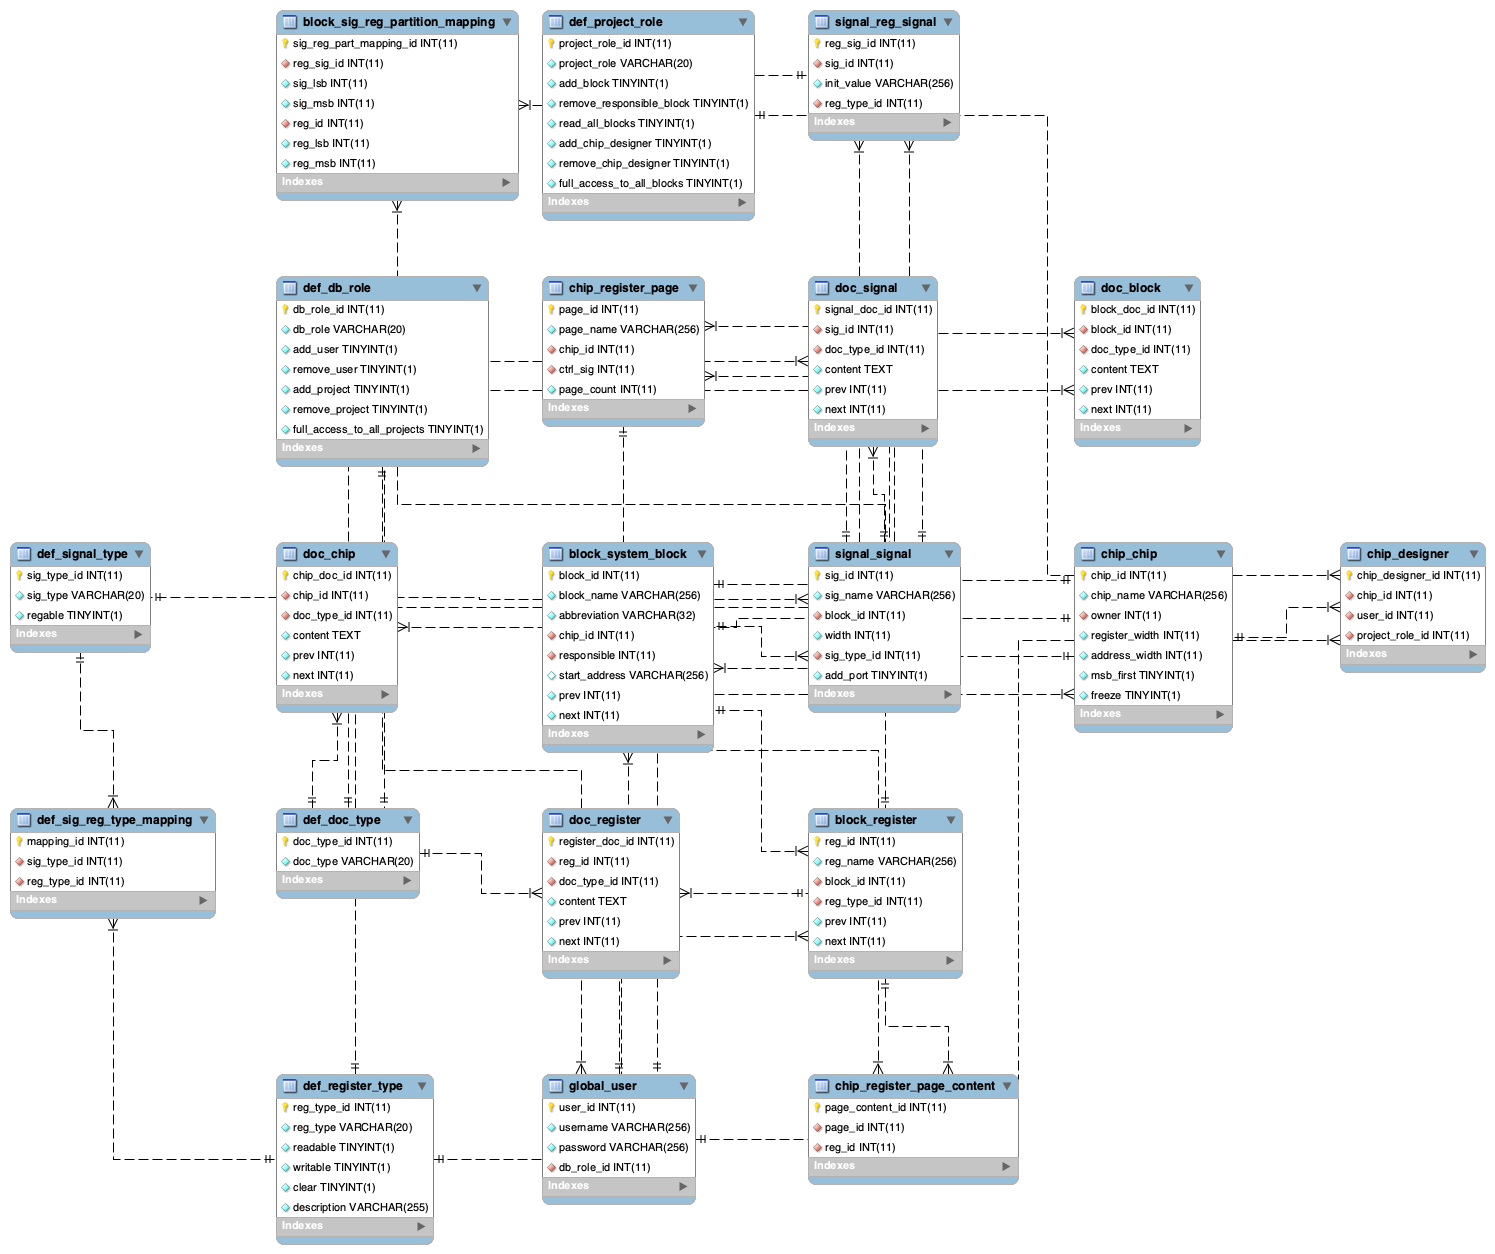
\includegraphics[width = \textwidth]{database}
\caption{Database Structure\label{fig:Database Structure}}
\end{figure}

It is important that we do not hardcode e.g. project roles and register types in the software. Instead, they are defined in the tables starting with \textbf{def} and this provides us much flexibility. For example, we can add a new project role by simply adding a new row to the \textbf{def\_project\_role} table without modifying the software itself.